\documentclass{ctexart}
\usepackage{graphicx}
\usepackage{amsmath}
\usepackage{amssymb}
\usepackage{hyperref}
\usepackage{geometry}
\usepackage{enumitem}
\usepackage{booktabs}
\usepackage{minted}
\geometry{a4paper, left=1in, right=1in, top=1in, bottom=1in}

\title{《深度学习基础》第三次实验报告}
\author{PB24000150 李欣宸}
\date{\today}

\begin{document}

\maketitle

本文是《深度学习基础》的第三次实验报告。代码实现在 \verb|lab/lab3| 目录下，报告内容包含要求中的必做内容和 3 个附加实验：手动实现 MHA、位置编码分析和自回归 MHA。对应实现主要在 \verb|model.py| 的 \verb|MultiHeadSelfAttention|、\verb|RotaryPositionalEncoding| 和因果 mask 分支中。所有实验记录都可在 \url{https://wandb.ai/xinchengo-ustc/ai3003-lab3} 上找到。

本实验主要在 \url{https://modal.com} 的 GPU 上进行训练，该网站为函数式计算平台，有每月 \$30 的免费额度，非常推荐大家使用。

我没有做可视化分析和超参数调优分析，因为对一个退化的 Transformer 来说这些分析意义不大。

在实验要求之外，我进行了“基线模型分析”，在实验报告“结果与讨论”中对应“基线分析”部分。


\section{实验设计}

\subsection{实验设置} \label{sec:experimental-setup}

\paragraph{数据集}
本实验使用 IMDB 电影评论情感分类数据集，共 50000 条电影评论。数据经过 \verb|utils.py| 中的 \verb|split_csv_data()| 随机打乱后划分为训练、验证和最终评测三部分，比例为 $0.72:0.08:0.20$，对应 36000 条训练样本、4000 条验证样本和 10000 条最终评测样本；标签为二分类。

\paragraph{文本预处理}
文本预处理使用统一的 normalization scheme：先去除重音并转换为小写，再将非字母数字字符替换为空格。实验中使用基于 Huggingface Tokenizers 库的 BPE tokenizer，词表大小 16384，截断长度 256，在左侧填充 \verb|<pad>| 词元。

\paragraph{模型架构}
本实验使用的 Transformer 分类器为 2 层、4 头、隐藏层大小 128、全连接层大小 256 的轻量级 Transformer；训练时 mask 掉 \verb|<pad>| 词元，Dropout 比例为 0.5。若计入未在分类任务中使用的语言模型输出头，参数量约为 4.46M；只计算分类前向实际使用的部分，参数量约为 2.36M（其中嵌入层约 2.10M，Transformer 层约 0.26M）。

\paragraph{训练设置}
主实验中，模型使用 AdamW 优化器 \cite{loshchilov2017decoupled}；Transformer 和 MLP 的学习率设置为 $10^{-3}$，RNN 的学习率设置为 $10^{-4}$。参数初始化中，注意力内部使用 Xavier 初始化 \cite{glorot2010understanding}，其他参数使用 Kaiming 初始化 \cite{he2015delving}；模型使用端到端训练，即通过文本输入预测标签，使用 \verb|BCEWithLogitsLoss| 优化二分类目标；学习率规划使用带预热的余弦衰减；具体的训练设置在 \verb|config.json| 中定义。

\paragraph{评价指标}
按照实验要求，模型主要使用 Accuracy 和 F1-score 进行评价。训练代码调用 \verb|sklearn| 计算 Accuracy、Precision、Recall 与 F1；报告中主要汇报 Accuracy 和 F1。

\subsection{文件结构}

\begin{itemize}[noitemsep]
    \item \verb|config.json|：实验配置文件；
    \item \verb|model.py|：模型实现，包含 Transformer 分类器、RNN 分类器和 MLP 分类器的实现，以及手写 MHA、位置编码和自回归 MHA；
    \item \verb|tokenizer.py|：文本预处理和 tokenizer 实现文件，包含字符级、单词级和 BPE tokenizer 的实现；
    \item \verb|trainer.py|：训练脚本；
    \item \verb|modal_train.py|：主实验训练脚本，负责在 Modal.com 的 GPU 服务器上运行训练；
\end{itemize}

\subsection{实验原理}

\subsubsection{多头自注意力}

多头自注意力（Multi-Head Self-Attention, MHA）\cite{vaswani2017attention} 是 Transformer 模型的核心组件。具体来说，比起传统的 Attention \eqref{standard-attention}，多头自注意力将输入词元向量映射到多个子空间中进行计算，每个子空间对应一个“头” \eqref{multi-head-attention-detail}，最后将各头的输出拼接并线性变换得到最终的输出 \eqref{multi-head-attention}。

\begin{gather}
\allowdisplaybreaks
\operatorname{Attn}(Q, K, V) = \operatorname{softmax}\left(\frac{QK^T}{\sqrt{d_k}}\right)V,\quad Q = XW_Q, K = XW_K, V = XW_V \label{standard-attention} \\
\operatorname{MHA}(X) = \operatorname{Concat}(\operatorname{Attn}_1, \cdots, \operatorname{Attn}_h)W_O \label{multi-head-attention} \\
\operatorname{Attn}_i = \operatorname{Attn}(Q^{(i)}, K^{(i)}, V^{(i)}),\quad Q^{(i)} = XW_Q^{(i)}, K^{(i)} = XW_K^{(i)}, V^{(i)} = XW_V^{(i)} \label{multi-head-attention-detail}
\end{gather}

从参数量分析，单头注意力中 $W_Q,W_k,W_V \in \mathbb R^{d_\text{model} \times d_v}$，总参数量为 $3 d_\text{model} d_k$。而多头注意力总参数量为 $3 h d_\text{model} \frac{d_k}{h} = 3 d_\text{model} d_k$，加上输出线性变换 $W_O \in \mathbb R^{d_\text{model} \times d_\text{model}}$，总参数量为 $3 d_\text{model} d_k + d_\text{model}^2$，与单头注意力增加开销不大。

核心代码如下，详见 \verb|model.py| 中的 \verb|MultiHeadSelfAttention| 类。

\begin{minted}[frame=single]{python}
B, N, D = x.size()
Q, K, V = x @ self.W_Q, x @ self.W_K, x @ self.W_V
# (B, N, D) -> (B, N, num_heads, D_h) -> (B, num_heads, N, D_h)
(Q, K, V) = (
    t.view(B, N, self.num_heads, self.head_dim).transpose(1, 2)
    for t in (Q, K, V)
)
# 此处省略位置编码处理
attn_scores = Q @ K.transpose(-2, -1) / (self.head_dim ** 0.5)
# 此处省略因果 mask 处理
scores = torch.softmax(attn_scores, dim=-1)
output = scores @ V  # (B, num_heads, N, D_h)
output = output.transpose(1, 2).contiguous().view(B, N, D) @ self.W_o
\end{minted}


\subsubsection{旋转位置编码}

传统的位置编码 \cite{vaswani2017attention}（如正弦位置编码 \eqref{sinusoidal-pe}）通过为每个嵌入向量加上一个特定的向量来引入位置信息。

\begin{equation}
PE(p, 2i) = \sin\left(\frac{p}{10000^{2i/d_{model}}}\right), \quad PE(p, 2i+1) = \cos\left(\frac{p}{10000^{2i/d_{model}}}\right) \label{sinusoidal-pe}
\end{equation}

而旋转位置编码（Rotational Positional Encoding, RoPE）\cite{su2021rope} 则通过调整注意力机制，使注意力权重与词元间的相对位置有关，具体来说，\eqref{standard-attention} 只比较了 $Q$ 和 $K$ 各分量的相似性（通过内积），而 RoPE 对 $Q$ 和 $K$ 施加一个旋转变换；设 $Q = (\boldsymbol{q}_1, \boldsymbol{q}_2, \cdots, \boldsymbol{q}_N)^T$ 和 $K = (\boldsymbol{k}_1, \boldsymbol{k}_2, \cdots, \boldsymbol{k}_N)^T$，$\boldsymbol{q}_m$ 和 $\boldsymbol{k}_n$ 分别是第 $i$ 个词元的查询和键向量，将其视为复向量，则 RoPE 可用 \ref{rope-rotation} 表示：

\begin{gather}
\tilde{\boldsymbol{q}}_m = (q_0 + q_1 j, q_2 + q_3 j, \cdots), \quad \tilde{\boldsymbol{k}}_n = (k_0 + k_1 j, k_2 + k_3 j, \cdots) \label{complex-embedding} \\
\hat{\boldsymbol{q}}_m^{(i)} = \tilde{\boldsymbol{q}}_m^{(i)} \cdot e^{j m \theta_{i}}, \quad \hat{\boldsymbol{k}}_n^{(i)} = \tilde{\boldsymbol{k}}_n^{(i)} \cdot e^{j n\theta_{i}} \label{rope-rotation}
\end{gather}

这样的内积就会引入一个关于位置差 $m-n$ 的旋转项：

\begin{equation}
\Re\left[\sum_i\hat{\boldsymbol{q}}_m^{(i)} \cdot \hat{\boldsymbol{k}}_n^{(i)*}\right] = \Re\left[\sum_i\tilde{\boldsymbol{q}}_m^{(i)} \cdot \tilde{\boldsymbol{k}}_n^{(i)*} \cdot e^{j (m-n) \theta_{i}}\right] \label{rope-attention}
\end{equation}

这个比正弦位置编码在注意力机制中的相互作用更加自然。而且观察 \ref{rope-attention} 中的旋转项 $e^{j (m-n) \theta_{i}}$ 可以看出，当 $m-n$ 较小时，旋转较小，注意力作用方式与标准注意力更接近；当 $m-n$ 较大时作用方式与标准注意力差异更大；这使得 RoPE 更倾向于建立局部依赖关系，而在长距离下慢慢衰减，更类似自然语言的依赖模式 \cite{su2021rope}；但是，真实的模型中 RoPE 存在更复杂的作用机制 \cite{barbero2024rope}。

核心代码如下，详见 \verb|model.py| 中的 \verb|RotaryPositionalEncoding| 类。

\begin{minted}[frame=single]{python}
# 对 Q 和 K 都调用这个函数
def _rotate(self, x, sin_pos, cos_pos):
    # x: (B, Nh, N, Dh)
    x_even = x[..., 0::2]
    x_odd = x[..., 1::2]
    x_rot = torch.stack((
        x_even * cos_pos - x_odd * sin_pos,
        x_even * sin_pos + x_odd * cos_pos
    ), dim=-1)
    return x_rot.flatten(-2)
\end{minted}

\subsubsection{自回归 MHA}

普通的 self-attention 中，每个位置都可以看到整段序列。自回归注意力需要保证第 $i$ 个位置不能使用未来位置 $j>i$ 的信息，因此在 attention logits 上加入一个上三角 mask：

\begin{equation}
M_{ij} =
\begin{cases}
0, & j \le i, \\
-\infty, & j > i,
\end{cases}
\quad
\operatorname{Attn}_{\text{causal}}(Q,K,V)
= \operatorname{softmax}\left(\frac{QK^T}{\sqrt{d_k}} + M\right)V .
\end{equation}


核心代码如下，具体实现见多头自注意力部分。

\begin{minted}[frame=single]{python}
causal_mask = torch.triu(
    torch.ones(N, N, dtype=torch.bool, device=x.device),
    diagonal=1
)
attn_scores = attn_scores.masked_fill(causal_mask, float("-inf"))
\end{minted}

\section{结果与讨论}

\subsection{主实验结果}

训练在 Modal.com 上的远程服务器进行，表中汇报按验证集 Accuracy 选择的 best checkpoint。分词和 Transformer 设置参见 \ref{sec:experimental-setup}；RNN 使用 2 层双向 RNN，hidden dim 为 128。

\begin{table}[htbp]
    \centering
    \begin{tabular}{lccccc}
        \toprule
        配置 & best epoch & 验证集 Acc & 验证集 F1 & 测试集 Acc & 测试集 F1 \\
        \midrule
        Transformer + RoPE & 3 & 0.8830 & 0.8803 & 0.8833 & 0.8858 \\
        RNN & 8 & 0.8738 & 0.8709 & 0.8861 & 0.8888 \\
        \bottomrule
    \end{tabular}
    \caption{主实验模型结果}
    \label{tab:main-results}
\end{table}

\begin{figure}[htbp]
    \centering
    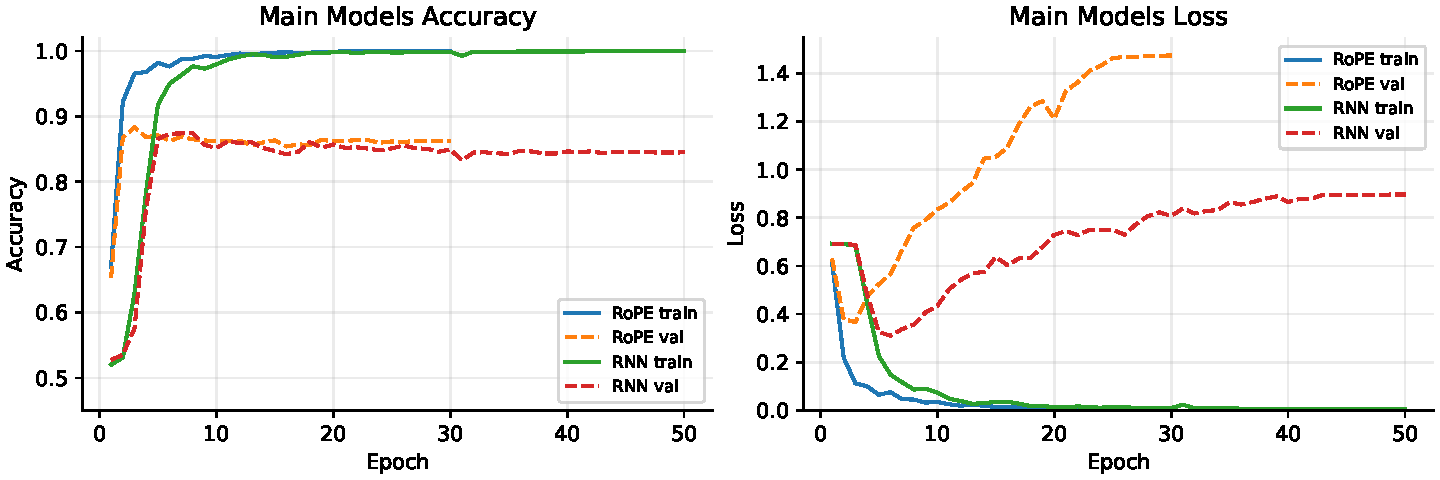
\includegraphics[width=0.95\linewidth]{figures/main_training_curves.pdf}
    \caption{主实验模型的训练曲线}
    \label{fig:main-training-curves}
\end{figure}

表 \ref{tab:main-results} 同时验证了附加实验 2 的手写 MHA 实现：模型没有调用 \verb|nn.MultiheadAttention|，而是用显式的 $W_Q,W_K,W_V,W_O$ 参数和矩阵乘法完成多头注意力。可以看到，Transformer 和 RNN 在测试集上的表现接近。需要注意的是，参见 \ref{sec:baseline-analysis} 中的结论，该结果并不能反映 Transformer 和 RNN 在语言建模能力上的差异。

从图 \ref{fig:main-training-curves} 可以看出，Transformer 和 RNN 都表现出明显的过拟合现象，但是 Transformer 的过拟合更早出现，且现象更为剧烈，这说明 Transformer 比起 RNN 具有更强的表示能力。
从训练效率看，Transformer 在较少 epoch 内就达到较高训练集 Accuracy，而 RNN 使用更小学习率并训练到 50 个 epoch，收敛速度更慢；不过在最终评测结果上，两者差距不大。

\subsection{位置编码分析}

附加实验 3 比较了无位置编码、正弦位置编码和 RoPE 三种方式。三组实验除位置编码外保持相同设置，均使用 \verb|bpe-hf-v14c8| tokenizer，结果见表 \ref{tab:positional-results}。

\begin{table}[htbp]
    \centering
    \begin{tabular}{lccccc}
        \toprule
        位置编码 & best epoch & 训练集 Acc & 训练集 F1 & 验证集 Acc & 验证集 F1 \\
        \midrule
        无位置编码 & 2 & 0.9347 & 0.9362 & 0.8762 & 0.8758 \\
        正弦位置编码 & 6 & 0.9574 & 0.9574 & 0.8818 & 0.8771 \\
        RoPE & 3 & 0.9653 & 0.9654 & 0.8830 & 0.8803 \\
        \bottomrule
    \end{tabular}
    \caption{位置编码方式对性能的影响}
    \label{tab:positional-results}
\end{table}

\begin{figure}[htbp]
    \centering
    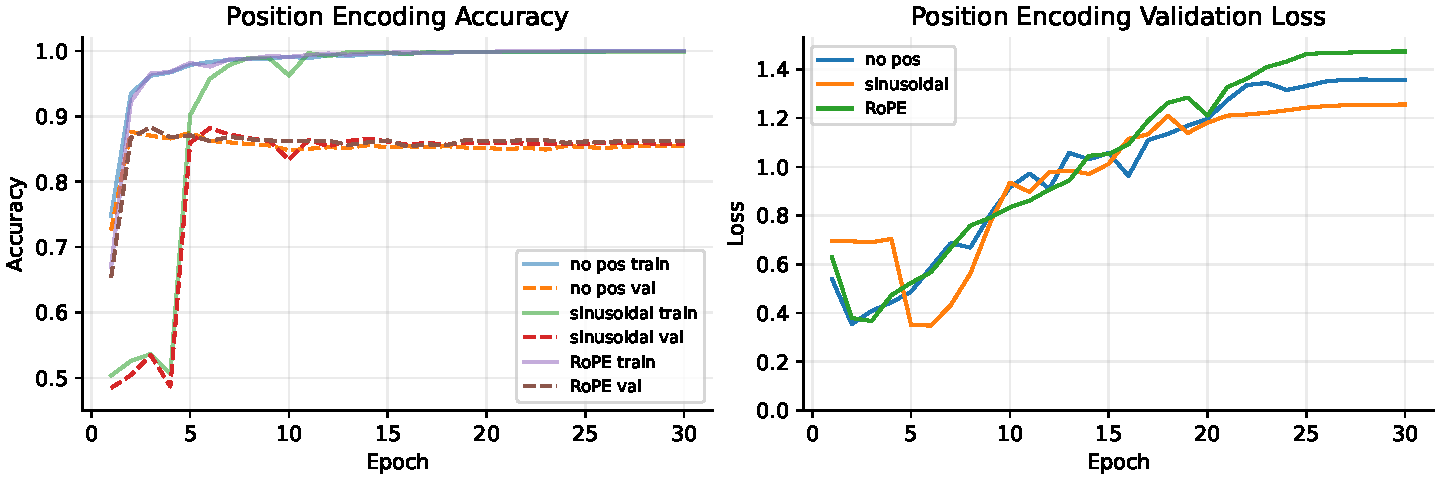
\includegraphics[width=0.95\linewidth]{figures/positional_training_curves.pdf}
    \caption{不同位置编码方式的训练曲线}
    \label{fig:positional-training-curves}
\end{figure}

同样的，由于 \ref{sec:baseline-analysis} 中的结论，这些结果也没有显著的意义，因为该实验的效果主要不是取决于位置编码而是出现词语以及词频特征。

不过图 \ref{fig:positional-training-curves} 中可以明显地看到，正弦位置编码的 loss 在前 5 个预热 epoch 中没有明显下降，而 RoPE 和无位置编码的 loss 在预热阶段就明显下降；这可能是因为正弦位置编码在注意力机制中的作用较为复杂，不像 RoPE 直接作为一个乘法因子，导致训练时，模型需要一段时间“适应”其引入的“噪声”。

\subsection{自回归 MHA}

附加实验 5 在 RoPE Transformer 上加入因果 mask，结果见表 \ref{tab:causal-results}。

\begin{table}[htbp]
    \centering
    \begin{tabular}{lcccc}
        \toprule
        注意力形式 & 训练集 Acc & 训练集 F1 & 验证集 Acc & 验证集 F1 \\
        \midrule
        非因果 MHA + RoPE & 0.9653 & 0.9654 & 0.8830 & 0.8803 \\
        自回归 MHA + RoPE & 0.9646 & 0.9647 & 0.8858 & 0.8819 \\
        \bottomrule
    \end{tabular}
    \caption{自回归 MHA 与普通 MHA 的对比}
    \label{tab:causal-results}
\end{table}

\begin{figure}[htbp]
    \centering
    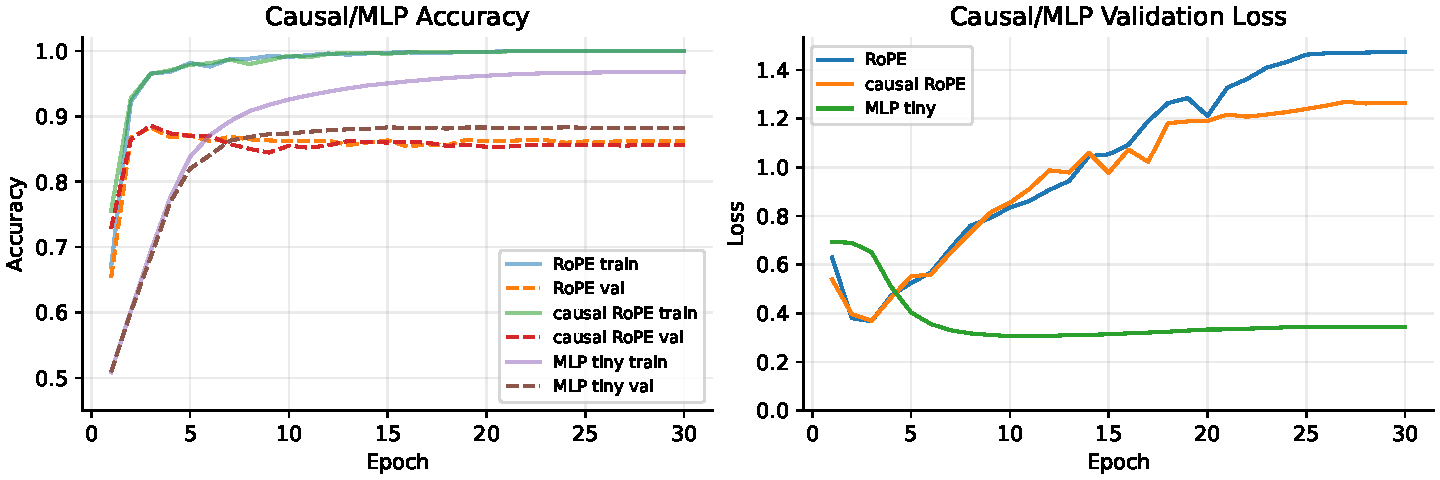
\includegraphics[width=0.95\linewidth]{figures/causal_baseline_training_curves.pdf}
    \caption{自回归 MHA 与基线模型的训练曲线}
    \label{fig:causal-baseline-training-curves}
\end{figure}

在该实验中，自回归 MHA 的训练和非自回归的训练曲线 \ref{fig:causal-baseline-training-curves} 和训练结果 \ref{tab:causal-results} 没有明显差异，这仍然是任务本身的性质 \ref{sec:baseline-analysis} 决定的。

\subsection{基线分析} \label{sec:baseline-analysis}

情感分析任务可以很好地用关键词判断，所以，模型在验证集上达到 85\% 以上的准确率并不能体现模型学到了多少真正的语言理解能力。

因此，我设计了基线模型（\verb|model.py| 中的 \verb|MLPClassifier|），它将所有词元的嵌入向量平均后输入一个 MLP 进行分类。对于 \verb|config.json| 中的 \verb|end2end-mlp-tiny| 配置中，嵌入维度为 32，MLP 唯一隐藏层的维度为 32；另外使用 \verb|Qwen3.5-2B| 的 zero-shot 分类结果作为另一个基线（\verb|test_qwen.py|）。结果见表 \ref{tab:baseline-results}。

\begin{table}[htbp]
    \centering
    \begin{tabular}{lcccc}
        \toprule
        模型 & 验证集准确率 & 验证集 F1 & 测试集准确率 & 测试集 F1 \\
        \midrule
        MLP（\verb|end2end-mlp-tiny|） & 0.8830 & 0.8802 & 0.8863 & 0.8882 \\
        Qwen3.5-2B (zero-shot) & -- & -- & 0.8995 & 0.8957 \\
        Transformer 分类器（正弦） & 0.8818 & 0.8771 & -- & -- \\
        Transformer 分类器（RoPE） & 0.8830 & 0.8803 & 0.8833 & 0.8858 \\
        \bottomrule
    \end{tabular}
    \caption{基线模型与 Transformer 模型的性能比较}
    \label{tab:baseline-results}
\end{table}

这个平均池化 MLP 大概可以理解为，给每个词分配 32 个特征，然后对所有词的特征取平均得到一个全局表示，再通过一层 32 维隐藏层的 MLP 输出二分类结果。即使是这种简单的模型，其训练结果也与 Transformer 分类器相当。
Qwen3.5-2B 只作为外部 zero-shot 参照，没有参与模型选择，因此这里只报告最终评测结果。

为了检查 MLP 是否只是指标相近，还是和 RoPE Transformer 在相同样本上犯错，我进一步对测试集逐样本比较二者预测，结果见表 \ref{tab:baseline-error-overlap}。

\begin{table}[htbp]
    \centering
    \begin{tabular}{lc}
        \toprule
        指标 & 数值 \\
        \midrule
        样本数 & 10000 \\
        RoPE Transformer 错误样本数 & 1167 \\
        MLP 错误样本数 & 1137 \\
        二者共同错误样本数 & 804 \\
        错误集合的 IoU & 0.5360 \\
        \bottomrule
    \end{tabular}
    \caption{MLP 与 RoPE Transformer 在测试集上的逐样本错误重合}
    \label{tab:baseline-error-overlap}
\end{table}

可以看到，MLP 的错误中有 70.7\% 也是 RoPE Transformer 的错误，RoPE Transformer 的错误中也有 68.9\% 同时被 MLP 分错，但错误集合并不完全相同；这说明 Transformer 部分退化为了一个类似于词袋模型的分类器，但学到的决策边界与 MLP 仍有差别。

\subsection{讨论}

该实验中数据规模小，且任务本身不需要复杂的语言理解能力，因此 Transformer，RoPE 等架构的优势无法体现出来；同时，模型的过拟合现象也非常明显。

但是我在实验中仍然观察到了正弦位置编码和 RoPE 在训练稳定性上的差异，以及 RNN 和 Transformer 在训练稳定性和学习率敏感性上的差异。

\section{结论}

本实验中，我主要收获了：

\begin{itemize}[noitemsep]
    \item 第一次书写了分为 \verb|model.py|、\verb|trainer.py| 和 \verb|tokenizer.py|、\verb|config.json| 的具有架构组织的训练代码，且核心部分（Transformer、位置编码和自回归 MHA）和架构设计为手写实现，锻炼了代码组织能力和编写能力；
    \item 使用 Modal.com 的函数式计算平台进行训练，体验了修饰器式的远程训练语法和按需分配的使用逻辑；
    \item 体会了在小数据和简单任务上，Transformer 和位置编码的优势无法体现出来，模型很容易退化为一个词袋模型；同时，过拟合现象非常明显；这说明了实验设计的重要性。
\end{itemize}

实验总体成功，最终模型在测试集上的准确率均在 88\% 以上，且训练过程稳定；虽然模型的表现并不能反映出 Transformer 和位置编码的优势，但是达到了预期的性能水平。

\begin{thebibliography}{9}

\bibitem{vaswani2017attention}
Vaswani, A., et al. Attention Is All You Need. NeurIPS, 2017.

\bibitem{loshchilov2017decoupled}
Loshchilov, I. and Hutter, F. Decoupled Weight Decay Regularization. ICLR, 2019.

\bibitem{glorot2010understanding}
Glorot, X. and Bengio, Y. Understanding the difficulty of training deep feedforward neural networks. AISTATS, 2010.

\bibitem{he2015delving}
He, K., et al. Delving Deep into Rectifiers: Surpassing Human-Level Performance on ImageNet Classification. ICCV, 2015.

\bibitem{su2021rope}
Su, J., et al. RoFormer: Enhanced Transformer with Rotary Position Embedding. arXiv:2104.09864, 2021.

\bibitem{barbero2024rope}
Barbero, F., et al. Round and Round We Go! What makes Rotary Positional Encodings useful? arXiv:2410.06205, 2024.

\end{thebibliography}

\end{document}
